\chapter{Colloidal Nanocrystal Synthesis} \label{sec:CQDSynthesis} \index{Quantum Dot:Colloidal} \index{Quantum Dot:Synthesis}

	The colloidal chemistry has offered a remarkable amount of tools for creating nanostructures. In the past growing simple spherical monodisperse
	nanoscrystals were the starting point of this research area, whereas nowadays various shapes, such as spheres, cubes, tetrapods,
	wires or rods can be engineered.
	The main advantages of the colloidal synthesis are:
	\begin{itemize}
		\itemsep 0pt
		\item High precision shape control of the crystal and Multicomponent structures are possible
		\item Good size adjustability, trough which the optical properties of the material are determined
		\item Monodispersity of the nanocrystals
		\item Low energy and low cost fabrication with simple experimental setup
		\item Broad range of materials, including metals, semiconductors and magnetic materials can be synthesized at sub-20nm range
	\end{itemize}
	Due to the listed advantages, the colloidal nanocrystal synthesis is the best candidate for commercial applications so far.
	
	\section{The synthesis}
		The colloidal nanocrystal synthesis is a wet chemical method to create nanostrucures. Its basic idea is the controlled growth of a nanocrystal,
		which is mainly depending on time.
		
		In figure \ref{fig:LaMer}, a reaction flask with thermometer and injection in form of a syringe is sketched. In praxis a heater is installed
		around the lower part of the flask, to keep the solvent at a desired constant temperature.
		
		The procedure itself starts with the heating of a solvent funneled into the flask. The thermometer will indicate the temperature of the solvent,
		which is a key variable for a good growth process. Therefore it is important to control, as the reaction will have an influence on the temperature
		as well.
		
		Once the solvent has reached the desired temperature, the growing of the nanocrystals is initiated, with the injection of precursors. From now on
		the duration of reaction determines the size of the final nanocrystal. The longer the reaction, the more the crystals will grow.
		The time to reach a desired size, are empirical values.
		
		As soon as the final size is reached, the reaction is stopped, by switching of the heating and cooling down the compound.
		
		After the reaction was stopped, the nanocrystals get washed in a last step to remove impurities from the reaction.
		
		
		Once the nucleation process is stared, the size of the nanocrystal is determined by the time,
		i.e. the longer the reaction, the larger the crystals can grow. Figure \ref{fig:LaMer} illustrates the stages of
		the traditional LaMer model by the U.S.-American chemist Victor LaMer. 
		\begin{figure}
			\centering
			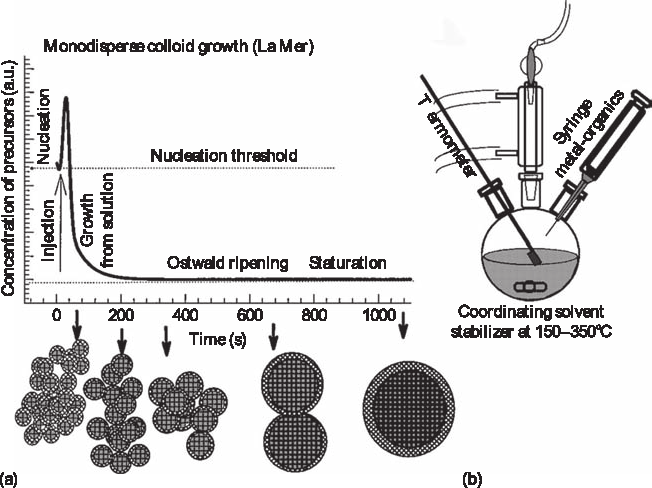
\includegraphics[width=0.5\textwidth]{Fig/LaMer.pdf}
			\caption{(a) Stages of the monodisperse nanocrystal synthesis according to La Mer. (b) Basic apparatus used in the synthesis. {\scshape Source:} \cite[p.4]{Klimov}}
			\label{fig:LaMer}
		\end{figure}
		Unfortunately, the process is more complicated, as the model predicts. It does not hold for hot-injection schemes for instance,
		because nucleation, ripening and growth may almost occur concurrently \cite[p.5]{Klimov}. Furthermore the nucleation process
		does not have to start immediately after injection, but it is usually a single discrete event in time
		
		three-component system composed of precursors, organic surfactants, and solvents	\\
		temperature high enough, precursors turn into monomers							\\
		if the concentration of the monomers in the reaction medium is high enough, crystal growth
		starts with nucleation process.																			\\
		
		Temperature critical factor for determining optimal crystal growth	\\
		Lower temperatures support growth process														\\
		Higher temperature causes annealing and rearrangement of atoms			\\
		Critical factors: monomer concentration
		
		
		The growth process of nanocrystals can occur in two different regimes, "focusing" and "defocusing" \\
		
		at high monomer concentrations, small critical sizes (size of nanocrystals stays the same) -> growth of
		nearly all particles (smaller particles grow faster than large ones) (since larger crystals need more atoms to
		grow than small crystals). 
		optimal when the monomer concentration is kept in a way, that present average nanocrystal size is always
		slightly larger than the critical size \\
		When the monomer concentration is depleted during growth, the critical size becomes larger than the average size present, and the
		distribution "defocuses" as a result of Ostwald ripening.
		
		
		beaker (Messbecher)
		